\section{Results}
\label{sec:results}

\paragraph{Queue-Haul beats the obvious heuristics, and the deadline is what decides.} The
real test of a planner is whether it outperforms simple baselines.
Figure~\ref{fig:baselines} sweeps the deadline and plots the share of KV-cache
\emph{bytes} that reach a destination in time, for our proportional-fair allocator
against six fixed heuristics and random placement. We weight by KV bytes, not job
count, since those bytes are the serving state we are trying to save, and a
plain count would hide a policy that helps many cheap sessions while abandoning enormous ones. Our allocator evacuates everything by $D{\approx}300$s. The
flexible heuristics (greedy, round-robin, state-only, random) get there too, but
only by ${\approx}600$s, twice the deadline. The two all-replay rules (replay-only
and least-loaded) never finish. They pour every rebuild onto the GPUs, hit the
prefill ceiling, and strand ${\sim}45\%$ of the KV cache even at $D{=}900$s.
Greedy even trails random at $D{=}300$s ($76\%$ vs.\ $90\%$), because chasing the
cheapest placement first hoards small sessions and leaves the expensive state
behind.

\begin{figure}[t]
\centering
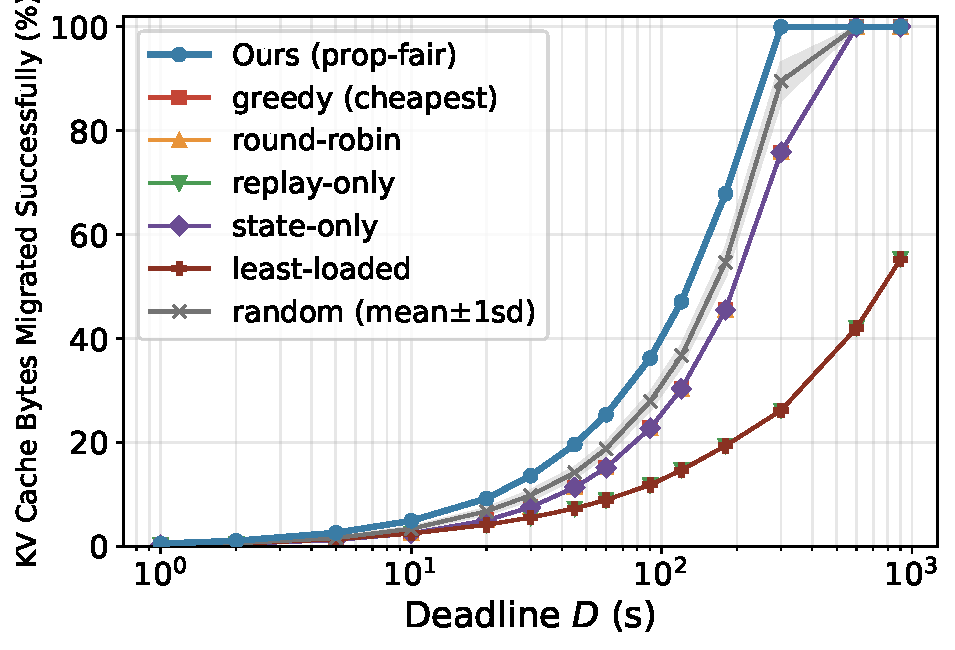
\includegraphics[width=\columnwidth]{kv_evacuated_baselines_vs_D.pdf}
\caption{Share of KV-cache bytes evacuated before the deadline, for our proportional-fair
allocator against six heuristics and random placement ($10$k sessions, band is
$\pm1$\,sd over seeds). Ours reaches $100\%$ by $D{\approx}300$s, the flexible
heuristics only by ${\approx}600$s, and the all-replay rules (replay-only,
least-loaded) stay prefill-bound near $55\%$.}
\label{fig:baselines}
\end{figure}

\paragraph{The rebuild mix is mostly replay, with a deliberate sliver of transfer.}
How does the optimizer actually rebuild each session? Figure~\ref{fig:mix} gives the
replay-versus-transfer split per model, for the fair allocation (Stage 1) and after
load balancing (Stage 2). Replay dominates. Stage 2 rebuilds $81$--$100\%$ of every
model's jobs by replay. Shipping $4$\,B/tok of context and recomputing is far lighter
on the inter-site link than moving tens of KiB/tok of KV cache, so replay spares the
network, the tight resource at these bandwidths. But the plan is never \emph{all}
replay, and that is the point. All-replay is exactly the prefill-bound failure of
Fig.~\ref{fig:baselines}. The optimizer keeps a minority of jobs on state
transfer, which leans on the idle state-ingest path rather than the GPUs, to stay
under the prefill ceiling. That small transfer band is what lets it reach $100\%$
where all-replay caps at $55\%$. Load balancing also \emph{sharpens} the choice.
Stage 2 lifts the replay share above the fair allocation's (DeepSeek V4 Pro
$45\%\!\to\!86\%$) and collapses its spread (wide Stage-1 error bars, tight Stage-2),
because the fair stage leaves the mix loosely pinned and peak-pressure settles it on
the network-sparing point.

\begin{figure}[t]
\centering
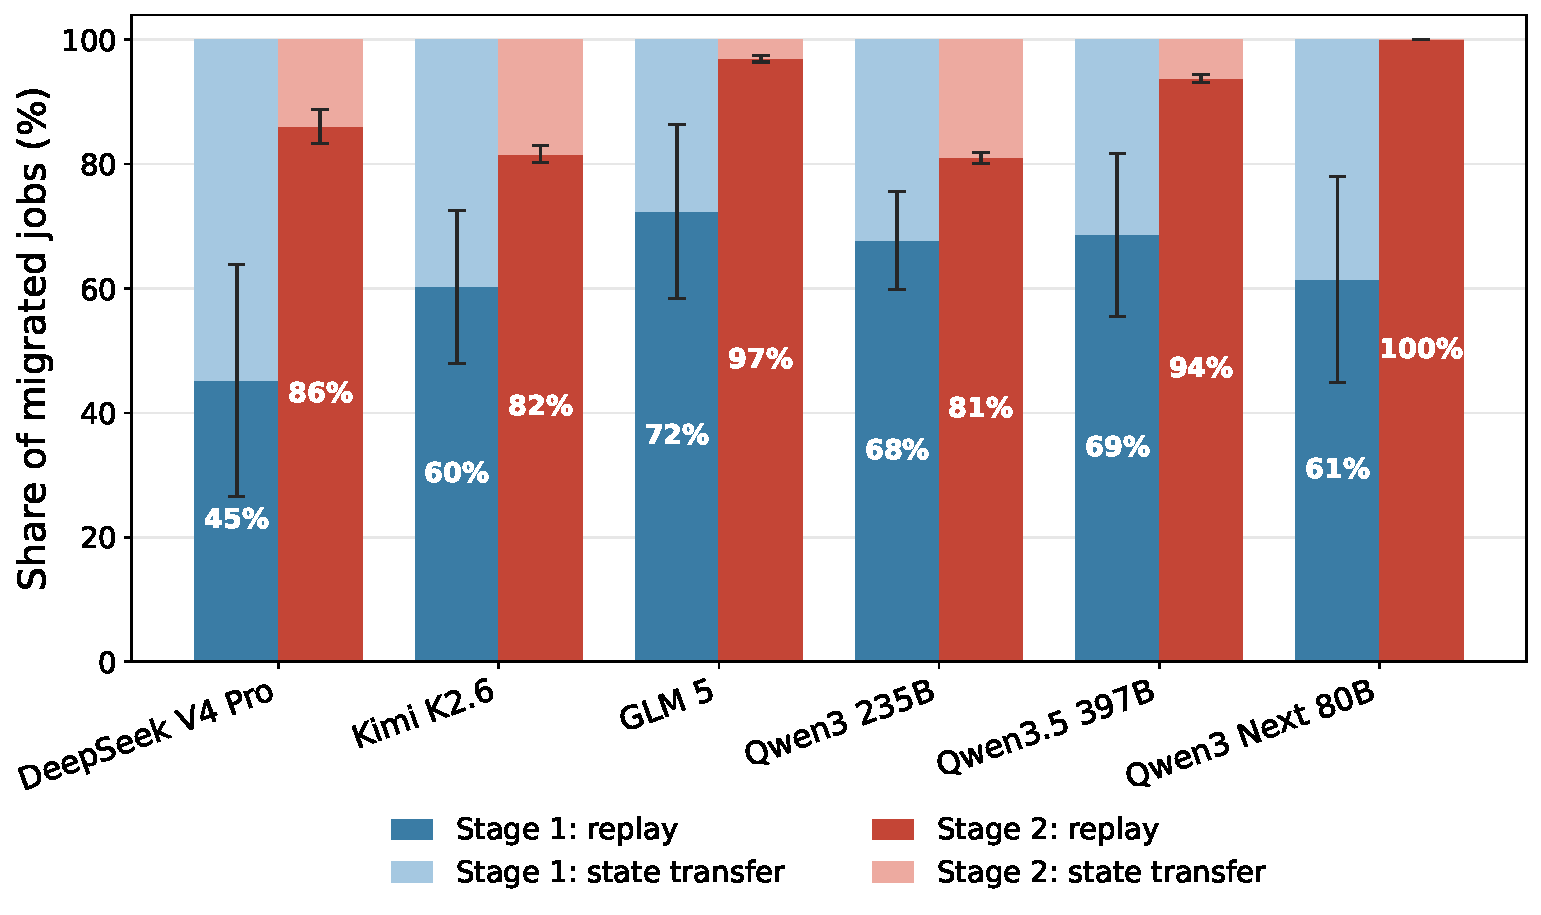
\includegraphics[width=\columnwidth]{stage2_action_mix.pdf}
\caption{Replay vs.\ state-transfer share of migrated jobs, per model, for the fair
allocation (Stage 1) and after peak-pressure balancing (Stage 2), with error bars
$\pm1$\,sd over $50$ instances. Stage 2 rebuilds $81$--$100\%$ by replay and tightens
the Stage-1 spread.}
\label{fig:mix}
\end{figure}

\paragraph{Where the allocation is most sensitive.} The Stage-2 prices double as a sensitivity
report. By the envelope theorem (Sec.~\ref{sec:methods}) each price gives a
log-capacity sensitivity $\partial\phi^\star/\partial\ln C_i=-\pi_i\hat p_i$, so a
single LP solve says which resource to grow to relieve the peak. Table~\ref{tab:sens} reads it off for the base instance. The
inter-site network owns $81\%$ of the sensitivity, prefill the remaining $19\%$ (most
of it on Qwen3-235B, the model with the tightest prefill supply), and state-ingest
none at all, since its $512$\,GB/s pools sit so far from binding that adding more never
moves the peak. One mild surprise sits inside the network. The price tracks
\emph{capacity}, not scarcity, so the $50$\,GB/s Site~C, which the optimizer loads
the heaviest, is the most sensitive of the three. A $1\%$ capacity bump shifts
$\phi^\star$ by exactly the predicted amount (Site~C, $-0.431$ measured vs.\ $-0.430$
from the price), and the entries sum to the deadline sensitivity
$d\phi^\star/d\ln D=-\phi^\star$.

\begin{table}[t]
\centering
\begin{tabular}{lrr}
\hline
Resource & $\pi_i$ & $\partial\phi^\star/\partial\ln C_i$ \\
\hline
\textbf{Network} & $0.81$ & \\
\quad Site C ($50$\,GB/s) & $0.46$ & $-0.43$ \\
\quad Site A ($25$\,GB/s) & $0.23$ & $-0.22$ \\
\quad Site B ($12.5$\,GB/s) & $0.12$ & $-0.11$ \\
\textbf{Prefill} & $0.19$ & \\
\quad Qwen3 235B & $0.08$ & $-0.07$ \\
\quad Kimi K2.6 & $0.06$ & $-0.06$ \\
\quad other 4 models & $0.05$ & $-0.05$ \\
\textbf{Ingest} & $0.00$ & $0$ \\
\hline
\end{tabular}
\caption{Sensitivity of the peak utilization $\phi^\star$ to each resource (base
instance, $D{=}300$s, prop-fair Stage~1, $\phi^\star{=}0.93$). The dual price $\pi_i$
(shares sum to $1$) is the marginal congestion price, and the last column
$\partial\phi^\star/\partial\ln C_i=-\pi_i\hat p_i$ is the peak's response to a
fractional capacity change. The network sets the peak, and ingest never binds.}
\label{tab:sens}
\end{table}

\section{Conclusion}

As the relationship between datacenters and the grid becomes more strained, the need for intelligent load shedding and migration grows. This project studies a convex relaxation of the session migration problem, where a source site must move its active inference sessions to other sites before a deadline. For each session the decision is where it lands and how its serving state is rebuilt there. We show that the solution is model-, resource-, and deadline-aware, and that the dual of the resource-pressure stage yields interpretable congestion prices that predict sensitivity. Future work includes an online receding-horizon scheduler that uses these prices for real-time decisions, and an extension of the model to richer resource interactions and scheduling dynamics such as queueing and stochastic resource availability.
